\documentclass[11pt,a4paper]{article}
\usepackage[T1]{fontenc}
\usepackage[utf8]{inputenc}
\usepackage[spanish,es-nodecimaldot,es-noshorthands]{babel}
\usepackage{lmodern,microtype,titlesec}
\usepackage[a4paper,left=27mm,right=24mm,top=27mm,bottom=25mm,headheight=18pt]{geometry}
\usepackage{amsmath,amssymb,booktabs,longtable,tabularx,array}
\usepackage{graphicx,xcolor,enumitem,fancyhdr,tikz,pgfplots}
\pgfplotsset{compat=1.18}
\usetikzlibrary{arrows.meta,positioning,babel}
\usepackage{csquotes}
\usepackage[backend=biber,style=apa,sorting=nyt]{biblatex}
\addbibresource{references.bib}
\definecolor{navy}{HTML}{203247}
\definecolor{teal}{HTML}{782F3A}
\definecolor{light}{HTML}{EDF3F6}
\usepackage[hypertexnames=false,colorlinks=true,linkcolor=navy,citecolor=teal,urlcolor=teal]{hyperref}
\usepackage{bookmark}
\setlength{\parindent}{0pt}
\setlength{\parskip}{6pt}
\setlength{\emergencystretch}{2em}
\setlist{nosep,leftmargin=*}
\pagestyle{fancy}\fancyhf{}
\fancyhead[L]{\scriptsize\textcolor{muted}{UNIVERSIDAD NACIONAL DE INGENIERÍA}}
\fancyhead[R]{\scriptsize\textcolor{muted}{ROBÓTICA}}
\fancyfoot[L]{\scriptsize\textcolor{muted}{Trabajo parcial · Borrador 03 · 2026-2}}
\fancyfoot[R]{\thepage}
\newcommand{\pendiente}[1]{\par\noindent\textcolor{teal}{\textbf{Pendiente:} #1}\par}
\newcommand{\nota}[1]{\par\noindent\colorbox{light}{\parbox{\dimexpr\linewidth-2\fboxsep}{#1}}\par}

\definecolor{wine}{HTML}{782F3A}
\definecolor{muted}{HTML}{536170}
\renewcommand{\baselinestretch}{1.08}
\renewcommand{\arraystretch}{1.18}
\renewcommand{\headrulewidth}{.3pt}
\renewcommand{\footrulewidth}{.3pt}
\titleformat{\section}{\Large\bfseries\color{navy}}{\thesection}{.6em}{}
\titleformat{\subsection}{\large\bfseries\color{navy}}{\thesubsection}{.6em}{}
\hypersetup{pdftitle={Modelado y simulación cinemática de un robot antropomórfico de 3 GDL}}

\begin{document}
\begin{titlepage}
\centering
{\large\bfseries UNIVERSIDAD NACIONAL DE INGENIERÍA}\par
{\small Facultad de Ingeniería Industrial y de Sistemas\\Unidad de Posgrado}\par
\vspace{10mm}

\includegraphics[width=25mm]{../assets/logos/uni-logo.png}\par
\vspace{9mm}
{\small\color{muted}MAESTRÍA EN INTELIGENCIA ARTIFICIAL}\par
\vspace{11mm}
{\large\color{wine}\bfseries TRABAJO PARCIAL}\par
\vspace{7mm}
{\LARGE\bfseries\color{navy}Modelado y simulación cinemática de un robot antropomórfico de 3 GDL}\par
\vspace{7mm}
{\normalsize Estudio del manipulador VSL de Ramzy et al. (2024)}\par
\vfill
\begin{tabular}{rl}
\textbf{Curso:} & Robótica y Sistemas Autónomos\\
\textbf{Docente:} & Ing. Wilson Dennis Reyes Vásquez\\
\textbf{Autores:} & Josemanuel [apellidos]\\
& Melissa [apellidos]\\
& Jairzinho Santos Fajardo\\
& Renzo [apellidos]\\
& Kenny [apellidos]\\
\end{tabular}\par
\vspace{10mm}
Lima, Perú\\2026-2
\end{titlepage}
\pagenumbering{roman}
\tableofcontents
\clearpage
\pagenumbering{arabic}
\section{Introducción}
El análisis cinemático permite relacionar el movimiento de las articulaciones de un robot con la posición y la velocidad de su efector final. Constituye la base para estudiar configuraciones alcanzables, singularidades y estrategias de seguimiento de trayectorias.

El presente trabajo desarrolla los contenidos del parcial de Robótica y Sistemas Autónomos a partir del manipulador antropomórfico de tres grados de libertad descrito por \textcite{ramzy2024}. Se abordarán la cinemática directa, inversa y diferencial, el análisis de singularidades y el control cinemático, acompañados de implementación en Python y simulación \parencite{consigna2026}.

El objetivo es formular y comprobar el modelo cinemático mediante casos reproducibles. El documento presenta el artículo de referencia, desarrolla cada tema y reúne resultados y conclusiones.

\section{Resumen del artículo de referencia}
\textcite{ramzy2024} estudian un manipulador de tres grados de libertad con eslabones de rigidez variable, denominado VSL. El artículo presenta su modelado cinemático y dinámico, junto con una validación experimental realizada por los autores.

La descripción geométrica, los parámetros Denavit--Hartenberg y las dimensiones publicadas permiten construir el modelo utilizado en este trabajo: $l_1=0.04$ m, $l_2=0.29$ m y $l_3=0.24$ m. El desarrollo cinemático se realiza sobre esa geometría nominal. Los resultados de las simulaciones propias se distinguirán de las mediciones experimentales publicadas.

Las expresiones del artículo se contrastarán con las transformaciones homogéneas. Las diferencias identificadas se documentarán sin modificar parámetros para forzar coincidencias.

\section{Desarrollo}
\subsection{Modelo y convenciones}
El robot considerado posee tres articulaciones rotacionales: base, hombro y codo. Se utilizan $q=[\theta_1,\theta_2,\theta_3]^T$, metros, radianes, vectores columna y la base como referencia. Las dimensiones publicadas son $l_1=0.04$ m, $l_2=0.29$ m y $l_3=0.24$ m \parencite{ramzy2024}.

La secuencia de desarrollo sigue las clases: método geométrico, matrices homogéneas, Denavit--Hartenberg (DH), inversa, Jacobianos, singularidades, trayectorias y control. El ejemplo antropomórfico de la semana 7 tiene la misma estructura DH; se sustituyen sus dimensiones por las del paper \parencite{course7}. No se trasladan al VSL las dimensiones, límites ni mallas de los robots utilizados como ejemplos docentes.

Con $q=0$, los eslabones móviles se extienden sobre $+x$ a la altura $l_1$. Se define $c_i=\cos\theta_i$, $s_i=\sin\theta_i$, $c_{23}=\cos(\theta_2+\theta_3)$ y $s_{23}=\sin(\theta_2+\theta_3)$.

\subsection{Cinemática directa}
\subsubsection{Método geométrico}
La proyección radial y la altura relativa del efector son
\begin{equation}
\rho=l_2c_2+l_3c_{23},\qquad z_r=l_2s_2+l_3s_{23}.
\end{equation}
Por proyección sobre la base se obtiene
\begin{equation}
P_{03}=\begin{bmatrix}p_x\\p_y\\p_z\end{bmatrix}=
\begin{bmatrix}c_1\rho\\s_1\rho\\l_1+z_r\end{bmatrix}.
\end{equation}
$\rho$ es una coordenada radial con signo; $\sqrt{p_x^2+p_y^2}=|\rho|$.

\subsubsection{Transformaciones homogéneas y DH}
La construcción por rotaciones y traslaciones de la semana 4 se adapta al RRR mediante \parencite{course4}
\begin{align}
M_{01}&=R_z(\theta_1)T_z(l_1)R_x(\pi/2),\\
M_{12}&=R_z(\theta_2)T_x(l_2),\qquad
M_{23}=R_z(\theta_3)T_x(l_3),\\
M_{03}&=M_{01}M_{12}M_{23}.
\end{align}
La convención DH es $R_z(\theta)T_z(d)T_x(a)R_x(\alpha)$, con los parámetros:
\begin{center}\begin{tabular}{ccccc}\toprule
Trama & $\theta$ & $d$ & $a$ & $\alpha$\\\midrule
$0\to1$ & $\theta_1$ & $l_1$ & 0 & $\pi/2$\\
$1\to2$ & $\theta_2$ & 0 & $l_2$ & 0\\
$2\to3$ & $\theta_3$ & 0 & $l_3$ & 0\\\bottomrule
\end{tabular}\end{center}
El producto da
\begin{equation}
M_{03}=\begin{bmatrix}
c_1c_{23}&-c_1s_{23}&s_1&c_1\rho\\
s_1c_{23}&-s_1s_{23}&-c_1&s_1\rho\\
s_{23}&c_{23}&0&l_1+z_r\\
0&0&0&1
\end{bmatrix}.
\end{equation}
La columna de posición coincide con el método geométrico. El código compara también una implementación de transformaciones elementales con la función DH, y comprueba $R^TR=I$ y $\det R=1$. Se reconstruyen las matrices en lugar de propagar las inconsistencias tipográficas del artículo.

\subsubsection{Espacio de trabajo}
Como en la semana 7, se recorren combinaciones de ángulos y se calcula $P_{03}$ en cada una. Se emplean 21 valores por articulación, con rangos ilustrativos $[-140,140]^\circ$, $[-120,120]^\circ$ y $[-110,110]^\circ$: 9261 posiciones. Estos rangos son un escenario de estudio, no límites mecánicos documentados del VSL.
\begin{figure}[htbp]\centering
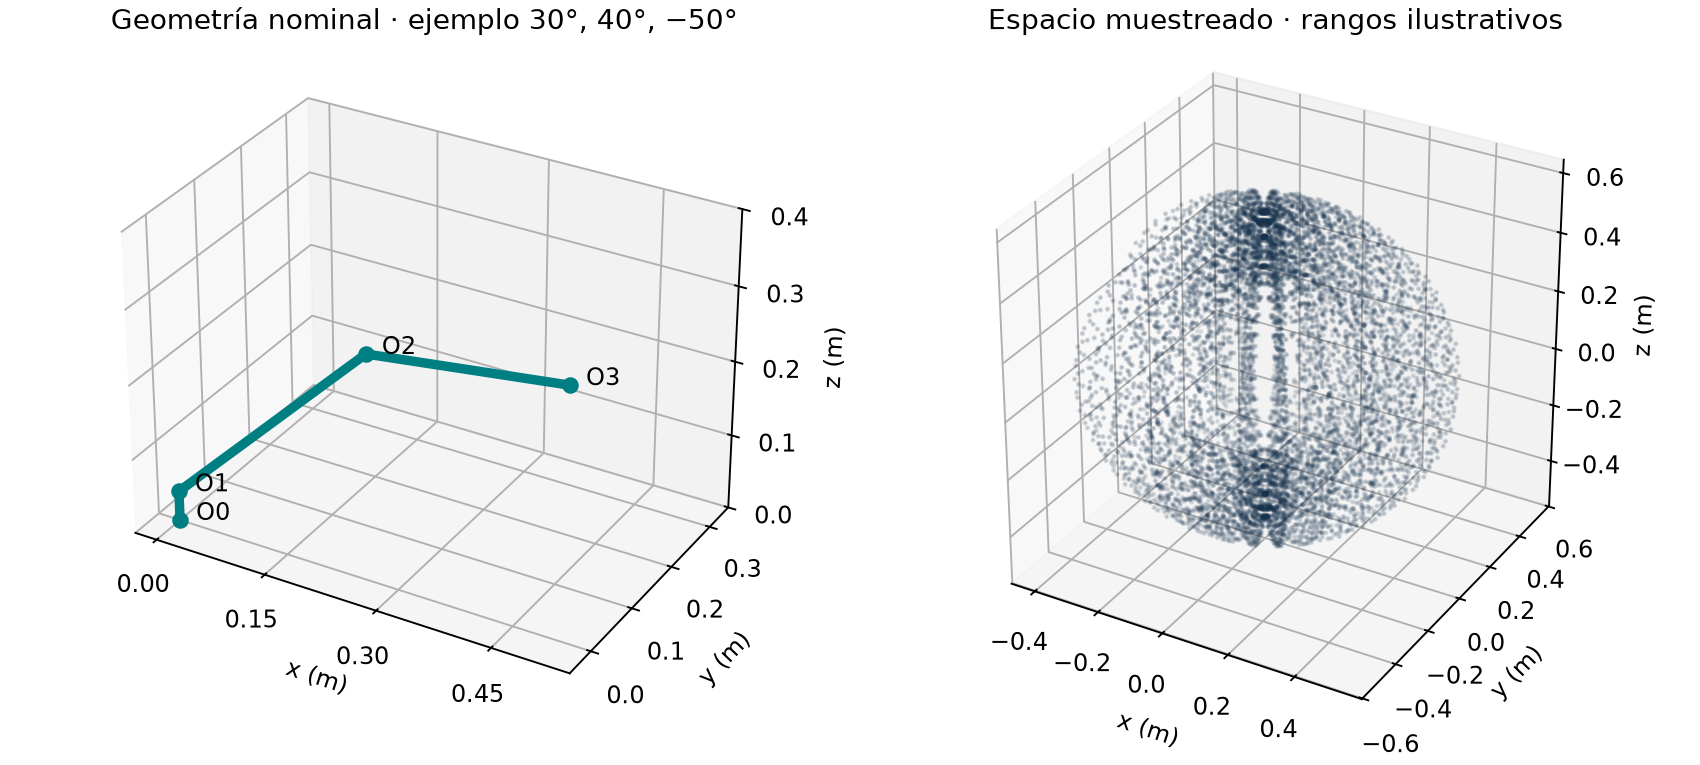
\includegraphics[width=\linewidth]{../simulations/course/results/run-001/workspace.png}
\caption{Geometría y espacio muestreado del modelo nominal. Elaboración propia.}
\end{figure}

\subsection{Cinemática inversa}
Se sigue la reducción geométrica de las semanas 5 y 7 \parencite{course5,course7}. Para un objetivo $(x,y,z)$, la distancia horizontal es $r=\sqrt{x^2+y^2}$ y la altura respecto del hombro es $h=z-l_1$. Fuera del eje, con $\phi=\operatorname{atan2}(y,x)$, dos pares de ángulo de base y proyección radial satisfacen $x=\rho\cos\theta_1$, $y=\rho\sin\theta_1$:
\begin{equation}
(\theta_1,\rho)=(\phi,+r)\quad\text{o}\quad(\phi+\pi,-r).
\end{equation}
El triángulo existe si $|l_2-l_3|\leq D\leq l_2+l_3$, con $D^2=r^2+h^2$. Para cada base se calculan el codo y el hombro mediante
\begin{align}
C_3&=\frac{D^2-l_2^2-l_3^2}{2l_2l_3},\qquad \theta_3=\pm\arccos C_3,\\
\theta_2&=\operatorname{atan2}(h,\rho)-
\operatorname{atan2}(l_3\sin\theta_3,l_2+l_3 C_3).
\end{align}
Para el punto $(0.333420,0.192500,0.291147)$ m, con coordenadas redondeadas, se obtienen cuatro ternas en grados:
\begin{center}
\begin{tabular}{rrrr}\toprule
$\rho$ (m) & Base & Hombro & Codo\\\midrule
$+0.385$ & 30 & 6.24 & 60\\
$+0.385$ & 30 & 60 & $-60$\\
$-0.385$ & $-150$ & 120 & 60\\
$-0.385$ & $-150$ & 173.76 & $-60$\\\bottomrule
\end{tabular}
\end{center}
Cada terna se verifica a precisión completa con las ecuaciones trigonométricas de posición y la traslación de $M_{01}M_{12}M_{23}$. En extensión o plegado coinciden las ramas de codo. Sobre el eje, cualquier base alcanza la misma posición y se elige un representante. La viabilidad física de cada postura requiere conocer los límites articulares y las colisiones.

\subsection{Cinemática diferencial}
\subsubsection{Jacobiano lineal por derivación}
El procedimiento de clase toma la posición de $M_{03}$ y deriva cada componente respecto de las variables articulares \parencite{course6,course7}:
\begin{equation}
\dot P_{03}=J_L(q)\dot q,\qquad
(J_L)_{ij}=\frac{\partial (P_{03})_i}{\partial\theta_j}.
\end{equation}
Por ejemplo, $\partial p_x/\partial\theta_1=-s_1\rho$, $\partial\rho/\partial\theta_2=-z_r$ y $\partial\rho/\partial\theta_3=-l_3s_{23}$. Por tanto,
\begin{equation}
J_L=\begin{bmatrix}
-s_1\rho&-c_1z_r&-l_3c_1s_{23}\\
c_1\rho&-s_1z_r&-l_3s_1s_{23}\\
0&\rho&l_3c_{23}
\end{bmatrix}.
\end{equation}
Las unidades de sus entradas son m/rad. El desplazamiento fijo $l_1$ desaparece al derivar. En el código, $J_L$ corresponde a la primera matriz devuelta por \texttt{jacobian}; la denominación anterior $J_v$ representa la misma matriz.

\subsubsection{Jacobiano angular y comprobación geométrica}
Para las tres articulaciones rotacionales, la semana 7 construye $J_\omega=[z_0\ z_1\ z_2]$, con ejes expresados en la base. En este modelo:
\begin{equation}
z_0=\begin{bmatrix}0\\0\\1\end{bmatrix},\quad
z_1=z_2=\begin{bmatrix}s_1\\-c_1\\0\end{bmatrix},\quad
J_\omega=\begin{bmatrix}0&s_1&s_1\\0&-c_1&-c_1\\1&0&0\end{bmatrix}.
\end{equation}
Así,
\begin{equation}
\begin{bmatrix}v\\\omega\end{bmatrix}
=\underbrace{\begin{bmatrix}J_L\\J_\omega\end{bmatrix}}_{J\in\mathbb R^{6\times3}}\dot q.
\end{equation}
Cada columna lineal también se obtiene de $z_{i-1}\times(P_{03}-o_{i-1})$. Las pruebas comparan ambas construcciones y verifican la parte angular mediante $[\omega]_\times=\dot R R^T$. Esta velocidad angular no equivale, en general, a derivar tres ángulos de Euler: esa parametrización utiliza un Jacobiano analítico diferente.

\subsubsection{Comprobación de velocidades}
Una trayectoria articular suave prescribe $q(t)$ y $\dot q(t)$. Se contrasta $J_L\dot q$ con la diferencia central $[P(t+\Delta t)-P(t-\Delta t)]/(2\Delta t)$. Para $\Delta t=0.01$ s, el error máximo es aproximadamente $3.99\times10^{-7}$ m/s. Al dividir el paso por dos, el error se reduce aproximadamente por cuatro, consistente con la diferencia central. Se excluyen los extremos del intervalo.
\begin{figure}[htbp]\centering
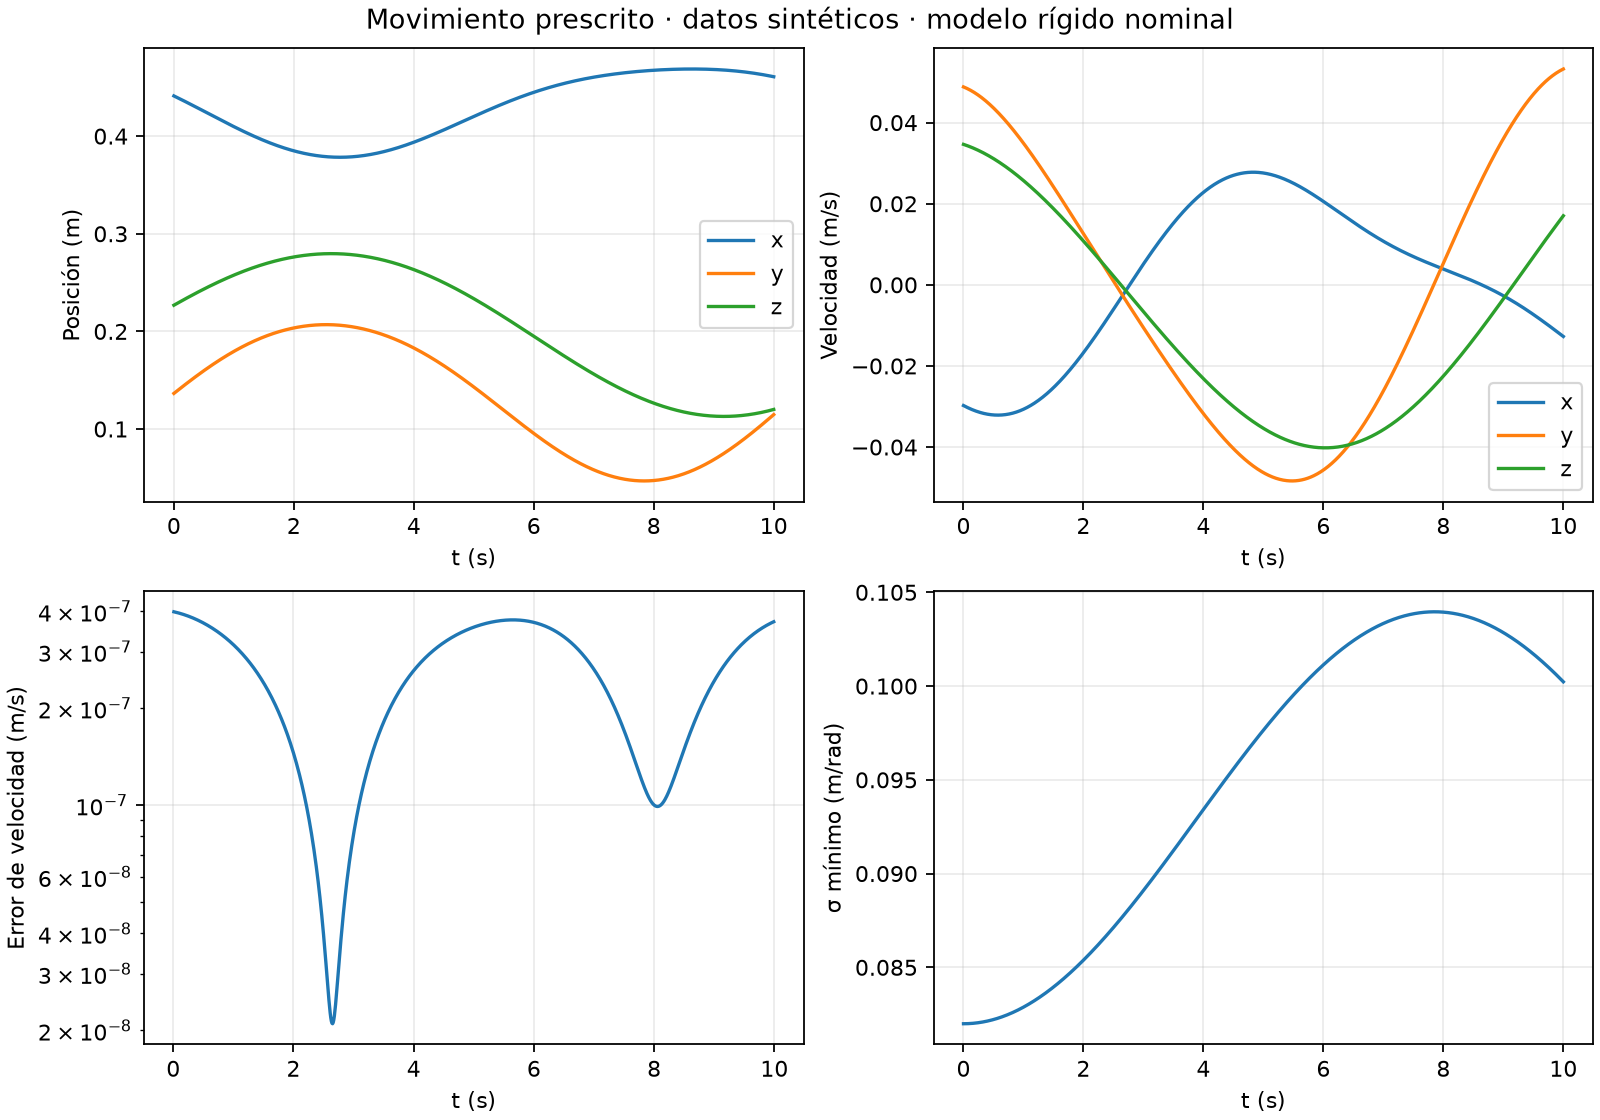
\includegraphics[width=.90\linewidth]{../simulations/differential/results/run-001/diagnostics.png}
\caption{Comprobación del Jacobiano lineal sobre movimiento prescrito. No corresponde a control en lazo cerrado.}
\end{figure}

\subsection{Singularidades}
\pendiente{El análisis incluirá el determinante, el rango y los valores singulares del Jacobiano de posición. Se estudiarán la alineación de eslabones y el eje de base, distinguiendo estas singularidades del rango del Jacobiano geométrico completo.}

\subsection{Control cinemático}
\pendiente{Se formulará una ley de seguimiento con trayectoria, ganancias, condiciones iniciales y límites definidos. La simulación evaluará errores, velocidades articulares y proximidad a singularidades en un escenario regular y otro exigente.}

\subsection{Resultados integrados y discusión}
\begin{center}\begin{tabularx}{\linewidth}{@{}lXX@{}}\toprule
Bloque & Métrica sugerida & Evidencia pendiente\\\midrule
Directa & Residuo DH frente a fórmula & Figuras y registro Python\\
Inversa & $\|p(q)-p_d\|$ & Ramas y casos inalcanzables\\
Diferencial & $\|J_v\dot q-\dot p_{FD}\|$ & Curvas y convergencia temporal\\
Singularidades & $\sigma_{\min}$ y rango & Casos regulares y singulares\\
Control & RMSE, máximo error, $\max|\dot q_i|$ & Trayectoria y sensibilidad\\\bottomrule\end{tabularx}\end{center}
\pendiente{Se presentarán resultados ejecutados, método de cálculo, versiones y límites. Se distinguirá la evidencia propia de los datos del paper y se analizará la discrepancia de su tabla 3.}

\section{Conclusiones}
\subsection{Cinemática directa}
\pendiente{Se sintetizará la relación entre las coordenadas articulares y la pose del efector, a partir del modelo desarrollado y sus comprobaciones.}
\subsection{Cinemática inversa}
\pendiente{Se resumirán las soluciones obtenidas, las condiciones de alcanzabilidad y los errores de reconstrucción.}
\subsection{Cinemática diferencial}
\pendiente{Se expondrá la correspondencia entre velocidades articulares y cartesianas, sustentada en la comparación del Jacobiano con derivadas numéricas.}
\subsection{Singularidades}
\pendiente{Se identificarán las configuraciones singulares y sus consecuencias para el movimiento del efector.}
\subsection{Control cinemático}
\pendiente{Se evaluará el seguimiento de trayectoria mediante errores, velocidades y comportamiento cerca de singularidades.}
\subsection{Conclusión general}
\pendiente{Se integrarán los hallazgos de los cinco temas y se precisarán el alcance y las limitaciones de los resultados obtenidos.}

\section{Recomendaciones}
\pendiente{Se propondrán mejoras sustentadas en los resultados: paso temporal, límites de operación, regularización y parámetros necesarios para ampliar el modelo.}

\clearpage
\printbibliography[heading=bibnumbered,title={Referencias}]
\appendix
\section{Esquema de marcos y relación entre métodos}
\begin{center}\begin{tikzpicture}[>=Stealth,scale=.9]
\coordinate (O0) at (0,0);\coordinate (O1) at (0,1.2);\coordinate (O2) at (2.2,2.5);\coordinate (O3) at (4.4,2);
\draw[very thick,navy] (O0)--node[left]{$l_1$}(O1)--node[above left]{$l_2$}(O2)--node[above]{$l_3$}(O3);
\foreach \p/\n in {O0/0,O1/1,O2/2,O3/3}{\fill (\p) circle(2pt);\node[below right] at (\p){$o_{\n}$};}
\draw[->] (O0)--++(0,1) node[left]{$z_0$};\draw[->] (O0)--++(1,0) node[below]{$x_0$};
\draw[->,wine] (O1)--++(1,0) node[right]{$x_1$};
\draw[->,wine] (O2)--++(.8,.48) node[above right]{$x_2$};
\draw[->,wine] (O3)--++(.85,-.19) node[right]{$x_3$};
\node[left] at (-.05,1.4){$z_1\odot$};\node[above] at (2.2,2.6){$z_2\odot$};
\end{tikzpicture}\end{center}
Vista esquemática del plano radial para $\theta_1=0$: $z_1$ y $z_2$ apuntan hacia fuera de la página ($-y_0$). El eje $x_1$ apunta radialmente; $x_2$ sigue la dirección del primer eslabón móvil y $x_3$ la del segundo. El efector está en $o_3$. La orientación de la base se recupera mediante $R_z(\theta_1)$.

\section{Archivos y reproducibilidad}
El PDF preparado se entrega junto a \texttt{main.tex}, sus secciones, bibliografía y figuras. El código se encuentra en \texttt{code/}; los parámetros, tablas y gráficas en \texttt{simulations/}. La guía \texttt{docs/reproduce.md} explica la reproducción opcional de los casos. Cada resultado conserva configuración y hashes. Los materiales docentes originales permanecen en \texttt{assets/utility/}, separados del código Python.

\end{document}
